% !TEX root = ../disertace.tex
%!TEX encoding = UTF-8 Unicode

\chapter{How are things in PDT 2.0}\label{PDT}
\label{sec:pdt}
\section{Prague Dependency Treebank}
\label{sec:pdt/pdt}
We work with the Prague Dependency Treebank (PDT, see \citealp{hajic:2005}), which is a large corpus with rich annotation on three layers: it has in addition to the morphological and the surface syntactic layers also the tectogrammatical layer.
(In fact, there is also one non-annotation layer, representing the ``raw-text'' segmented into documents, paragraphs, and tokens.)
Annotation of a sentence on the morphological layer consists of attaching several attributes to the tokens of the w-layer, the most important of which are morphological lemma and tag.
A sentence at the analytical layer is represented as a rooted ordered tree with labeled nodes. The dependency relation between two nodes is captured by an edge with a functional label.
The tectogrammatical layer has been construed as the layer of the (literal) meaning of the sentence and thus should be composed of monosemic lexemes and the relations between their occurrences.%
\footnote{With a few exceptions, such as personal pronouns (that refer to other lexeme) or coordination heads.}

On the tectogrammatical layer only the autosemantic words form nodes in a tree (t-nodes). Synsemantic (function) words are represented by various attributes of t-nodes. Each t-node has a lemma: an attribute whose value is the node's basic lexical form.
Currently t-nodes, and consequently their t-lemmas, are still visibly derived from the morphological division of text into tokens. This preliminary handling has always been considered unsatisfactory in FGD.%
\footnote{Functional Generative Description (FGD, \citealp{sgall-etal:1986,hajicova:1998}) is a framework for systematic description of a language, that the PDT project is based upon. In FGD units of the t-layer are construed equivalently to monosemic lexemes and are combined into dependency trees, based on syntactic valency of the t-nodes.}
There is a clear goal to distinguish t-lemmas through their senses, but %so far this process has only been completed for verbs and deverbative nouns and adjectives. 
this process has not been completed so far (see Section \ref{sec:pdt}).

Figure~\ref{fig:layers} shows the relations between the neighboring layers of PDT. 
\begin{figure}[htbp]
   \centering
   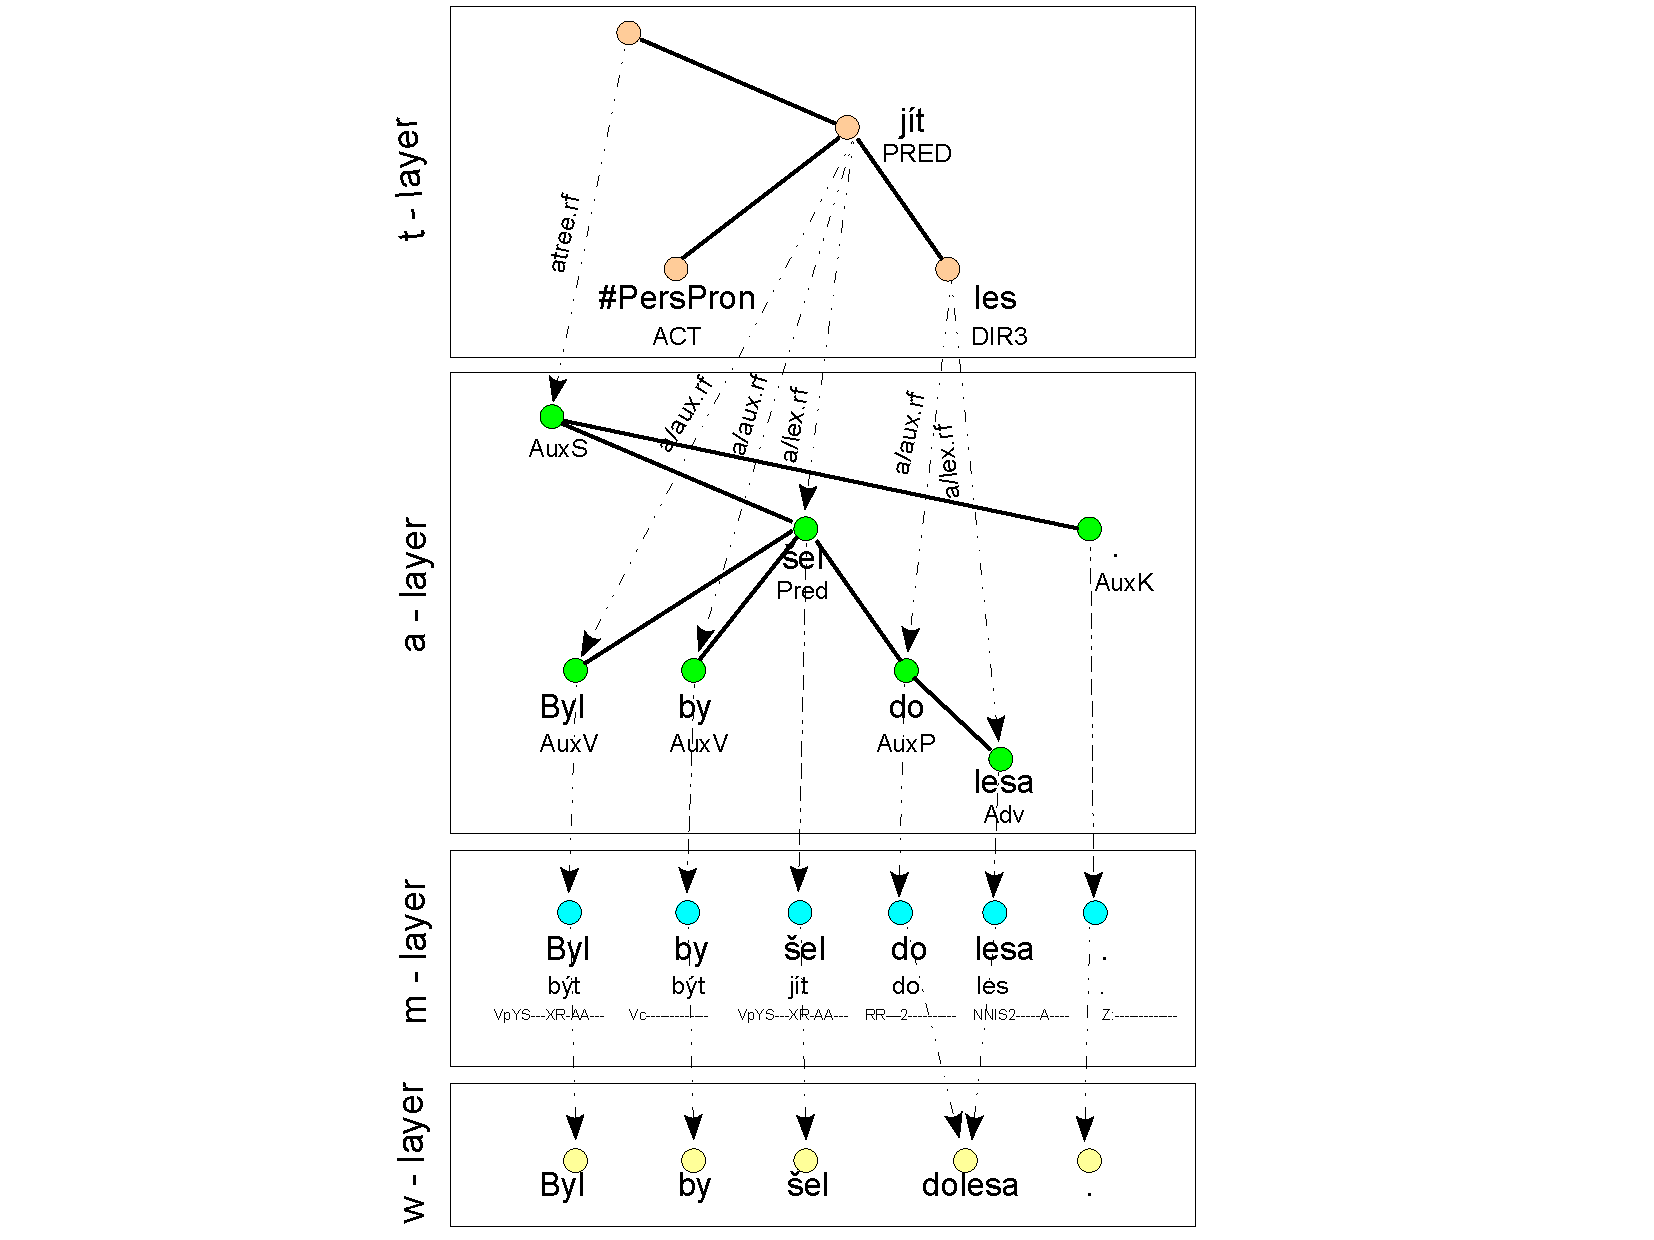
\includegraphics[scale=.38]{images/roviny.pdf} %180,0,580,595
%\begin{center}
%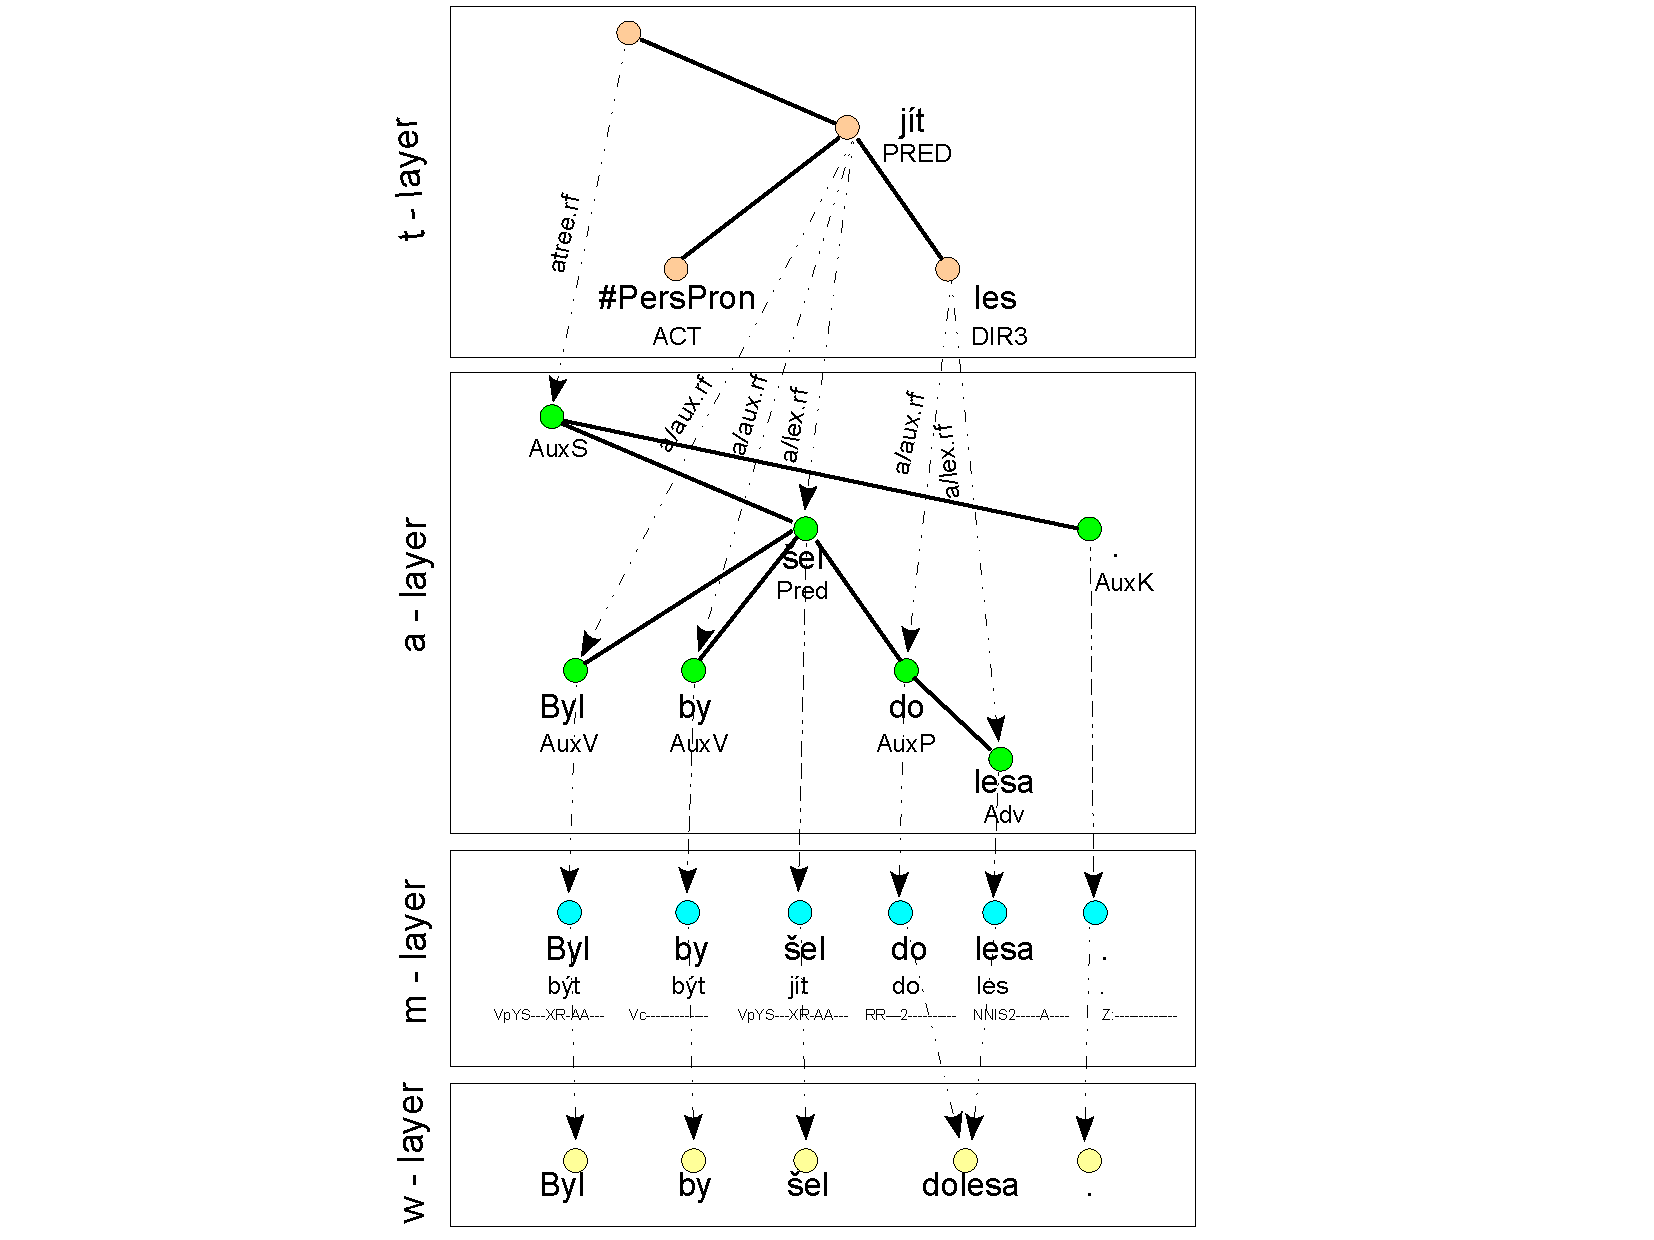
\epsfig{file=images/roviny.pdf,height=6cm,bbllx=100,bblly=425,bburx=300,
%        bbury=625,clip=}
%\end{center}
   \caption{The rendered Czech sentence \emph{Byl by šel dolesa}. (lit.: He-was would went toforest.) contains past conditional of the verb ``jít'' (to go) and a typo ``toforest'' repaired on m-layer.}
   \label{fig:layers}
\end{figure}

Our project aims at improving the current state of t-lemmas. Our goal is to assign each t-node a t-lemma that would correspond to a lexeme, i.e. that would really distinguish the t-node's lexical meanings. To achieve this goal, in the first phase of the project, which we report on in this paper, we \emph{identify multiword expressions and create a lexicon of the corresponding lexias}. A simple view of the result of our annotations is given in the Figure~\ref{fig:trees}, some technical details are in Section~\ref{sec:meth:annot}.
%Remaining t-lemmas of ``single-word t-nodes'' will be examined and possibly changed later. But to do that, we must finish the current phase in order to know what the remaining ``single-word'' nodes are.

% to leave out ???
%There are also other quite practical motivations for MWE annotation: If we want to identify coreference relations between for instance ``Association for Computational Linguistics'', ``ACL'', and  ``it'' in a text, we need to identify the first expression as a single unit. For some applications we might also need to know what kind of entity it is. 

\begin{figure}[htbp]
   \centering
   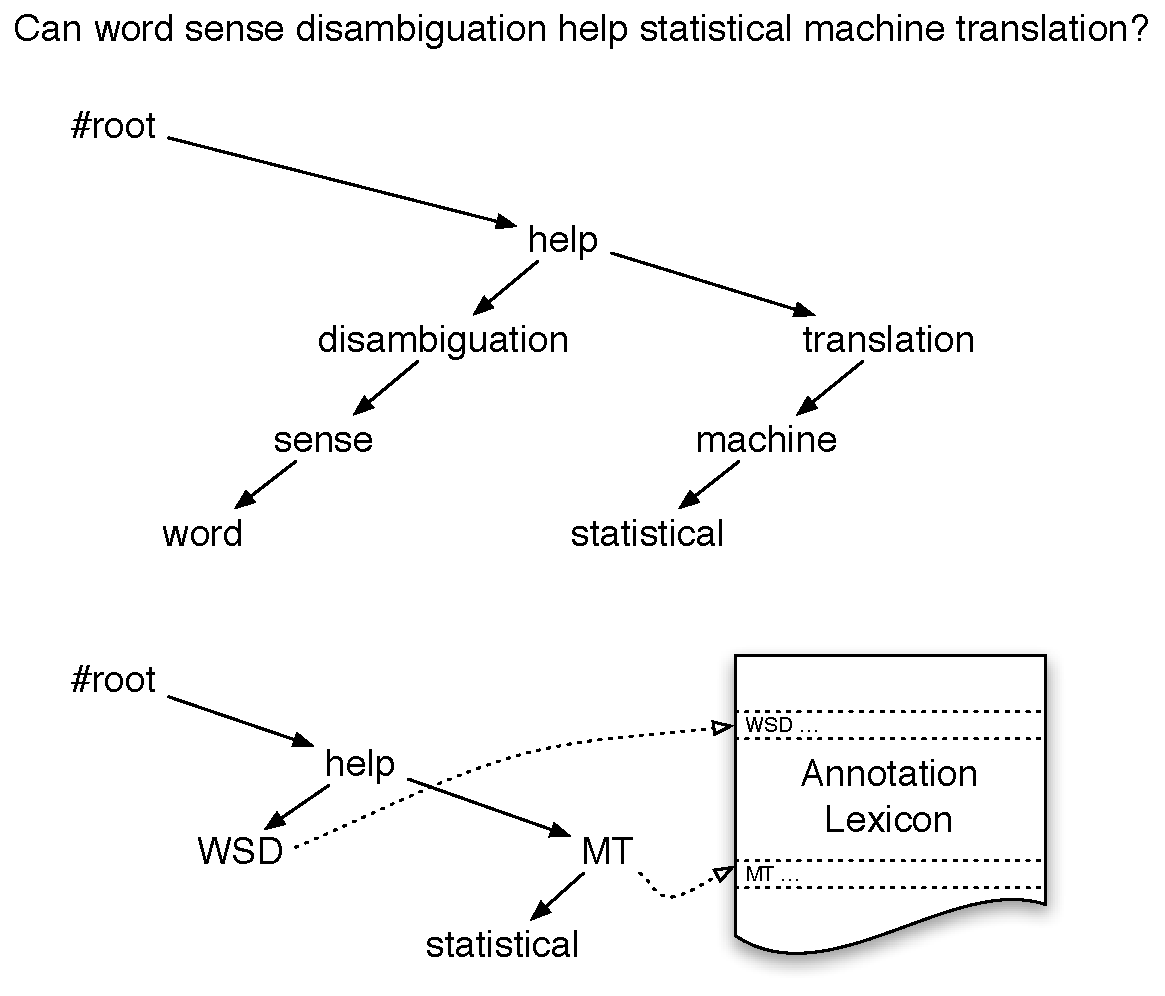
\includegraphics[width=3.4in]{images/stromecky.pdf}
   \caption{Schema of the changes in t-trees after integration of our annotations; every MWE forms a single node and has its lexicon entry}
   \label{fig:trees}
\end{figure}


In the Prague dependency treebank version 2.0 (PDT, ) there are several functors that refer to multiword expressions (MWEs) in one way or another. There are also two technical lemmas \texttt{\#Idph} and \texttt{\#Forn} that identify roots of subtrees representing MWE's. Tectogrammatical annotation is described in detail in~\citet{mikulova:2006}.


\section{Search and visualisation tools}

There are currently two graphical search engines for PDT: Netgraph \citep{mirovsky:2009} and TrEd \citep{pajas:tred}. Both have their respective benefits, but since TrEd is considerably faster due to its use of an SQL database backend \citep{pmltq}, we have used TrEd for all the examples in this work. We also give the search queries using the PML Tree Query language designed by \citet{pmltq} where appropriate.

%%%%%%%%%%
\section{List structures}

\subsection{Foreign Phrase: \code{t-node [t\_lemma = \#Forn]}}\label{PDT:Forn}
Foreign Phrase seems to be overused and its overuse seems a bit arbitrary. \\
- jmena firem jsou nekdy forn, nekdy ne. (dohledat)\\

%%
\subsubsection{Foreign phrases with just one t-node}
There are 34 occurrences of this construction in the PDT~2.0. Counting them is as easy as writing a query in Figure~\ref{fig:tq-forn1} and extending it with this filter: \code{>>count(\$n)}.

\begin{wrapfigure}{r}{0.32 \textwidth}
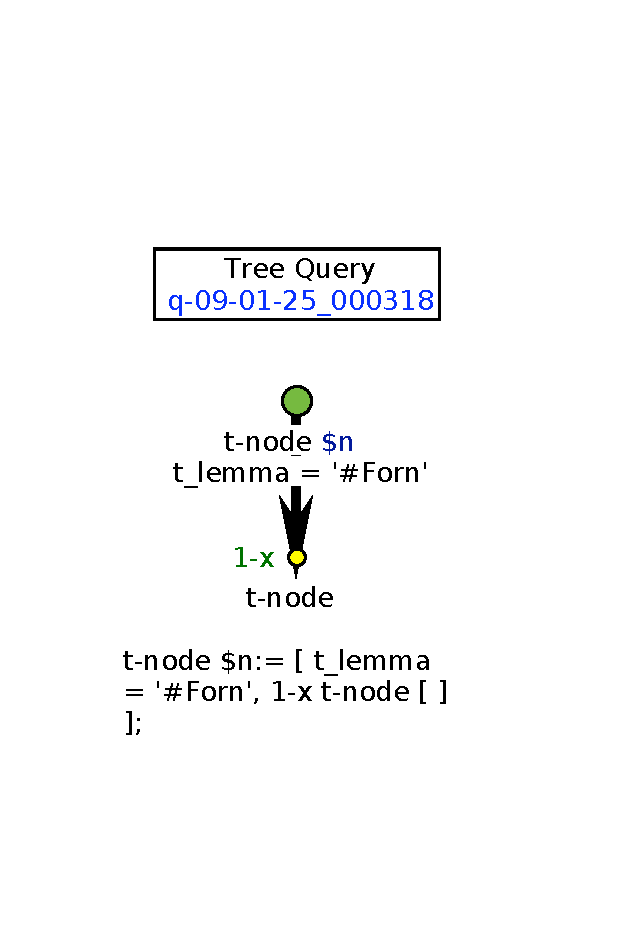
\includegraphics[width=0.3 \textwidth]{images/vyhledavky/query-forn-1-x.pdf}
\caption{PML-TQ search query for single-node foreing phrases}
\label{fig:tq-forn1}
\end{wrapfigure}

In case of the bibliographic reference in Figure~\ref{fig:forn-biblio} there is coordination of three foreign phrases corresponding to the parts of a bibliographic reference annotated, but the reason for this is not very clear. After all, the point of annotating foreign phrases as simple lists with a \code{\#Forn} node as a head was to make no assumptions about these pieces of a text \pageref{pdt-t-man:300}.  \\
- je to kvuli te interpunkci???

\begin{figure}[h]
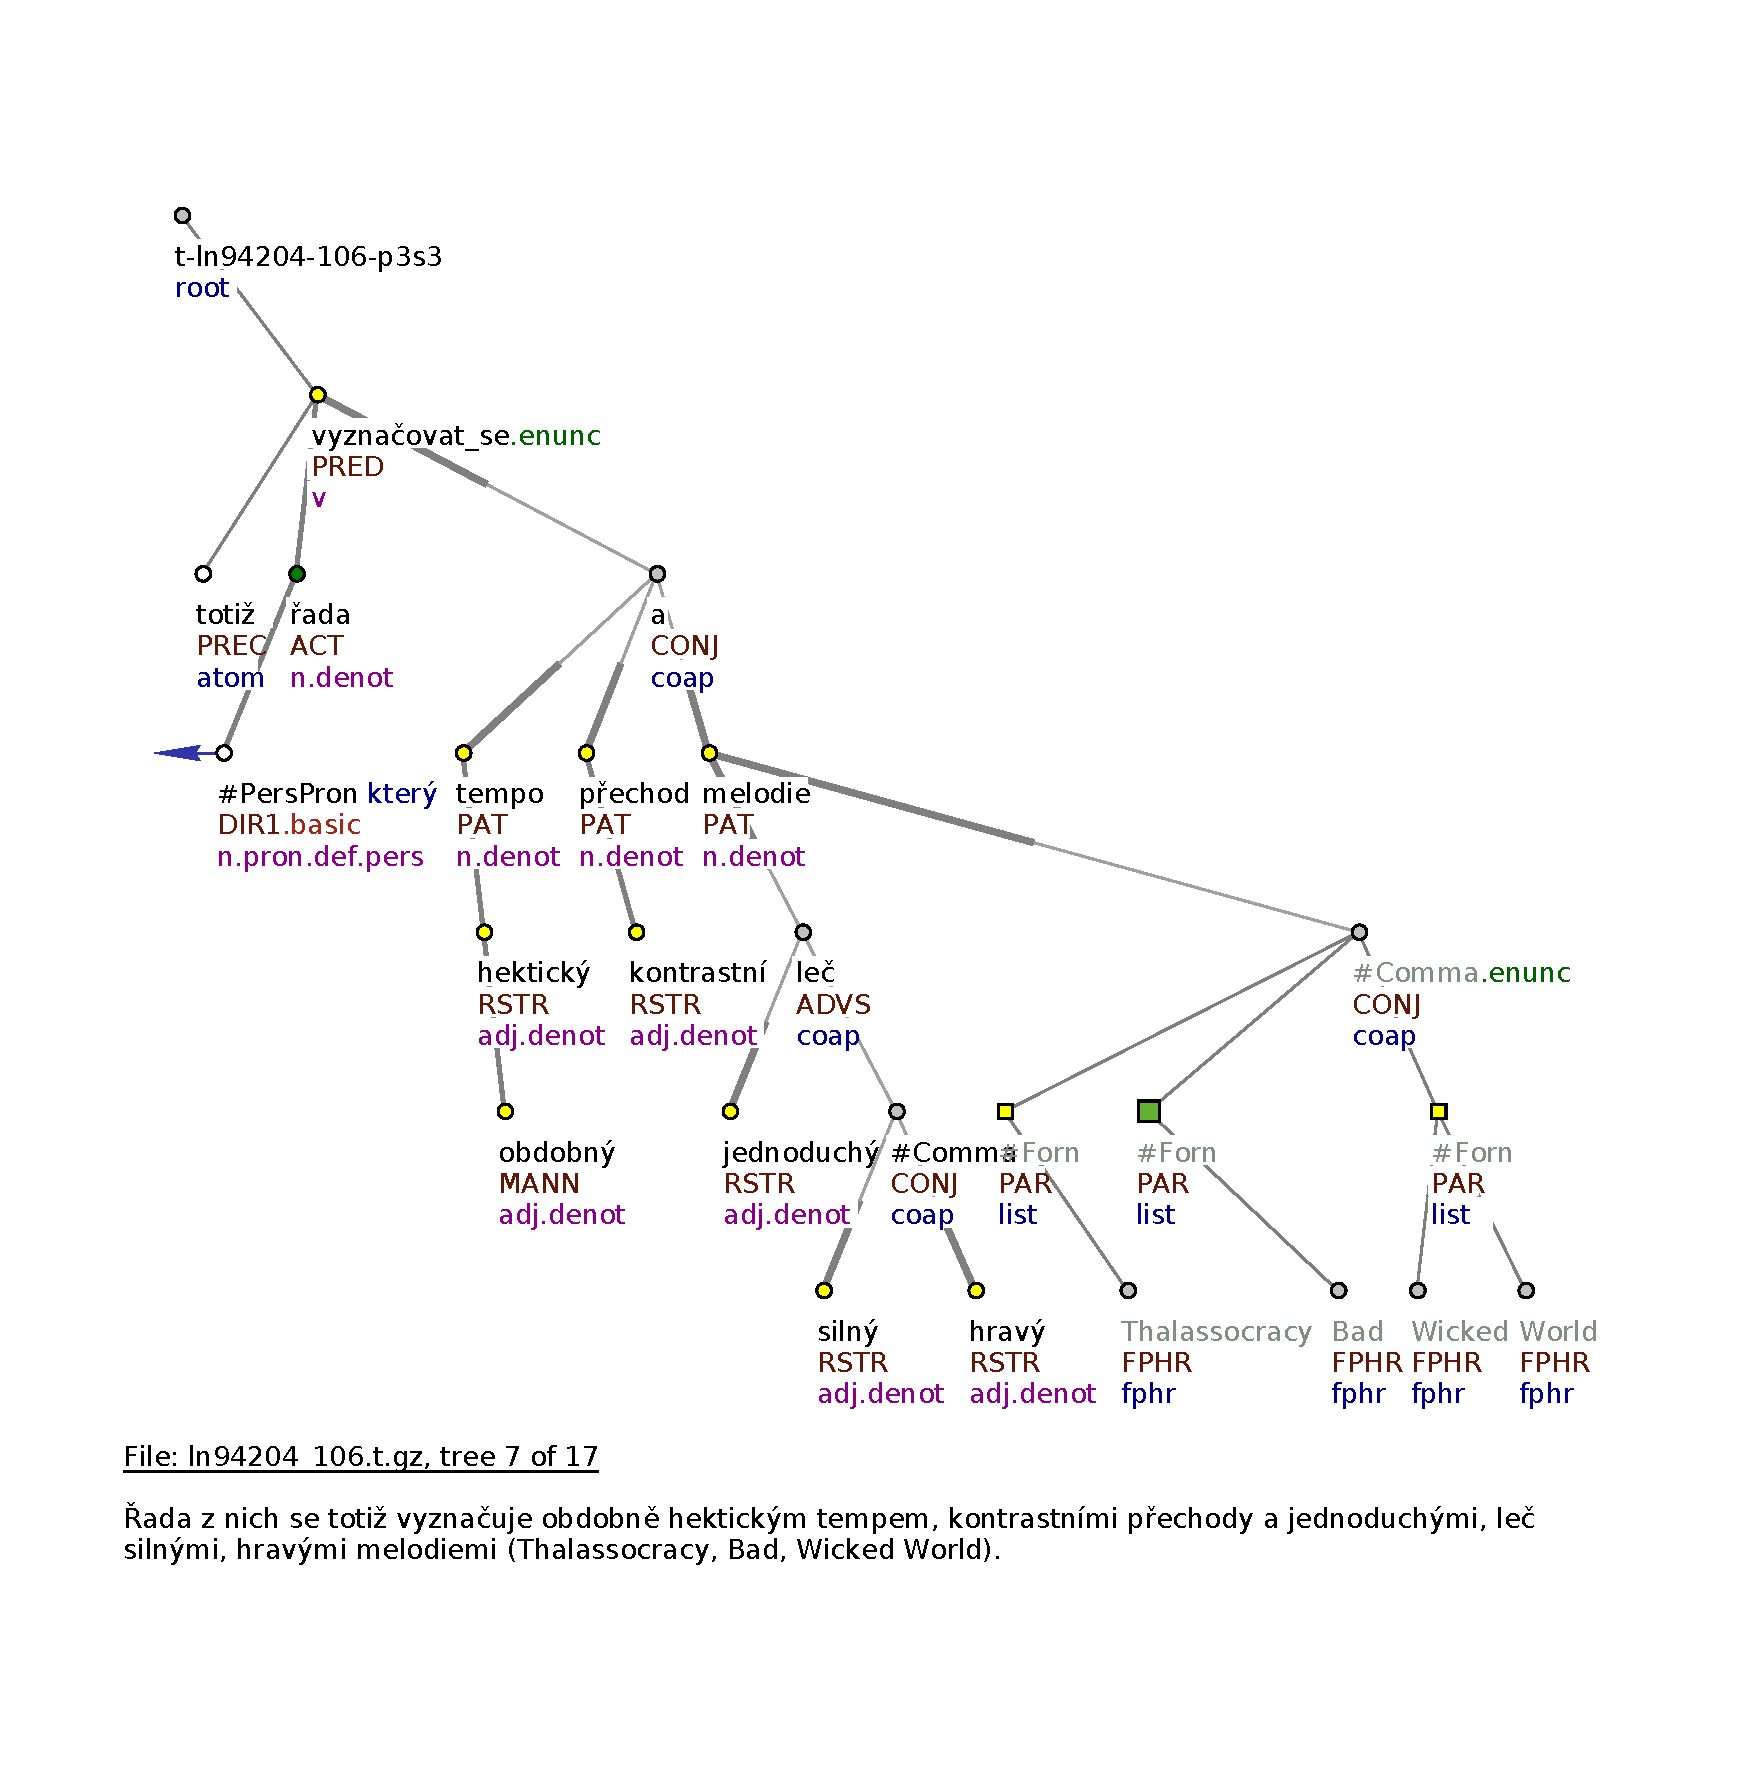
\includegraphics[width=\textwidth]{images/vyhledavky/forn-coord1x-biblio.pdf}
\caption{A bibliographic reference analysed as a coordination of three foreign phrases}
\label{fig:forn-biblio}
\end{figure}

Names of companies seem to be distinguished more by the country of origin then by any linguistic reasons, as demonstrated in Figure~\ref{fig:forn-firmy}. As far as linguistic criteria are concerned, Chemapol and Inekon are as foreign as Agip or Total. However the first two are, or at least were,%
\footnote{At the time of writing this thesis Chemapol is owned by another international company, which only emphasises vagueness of this distinction} %
%
Czech companies, while those in the latter group have a foreign origin.

\begin{figure}
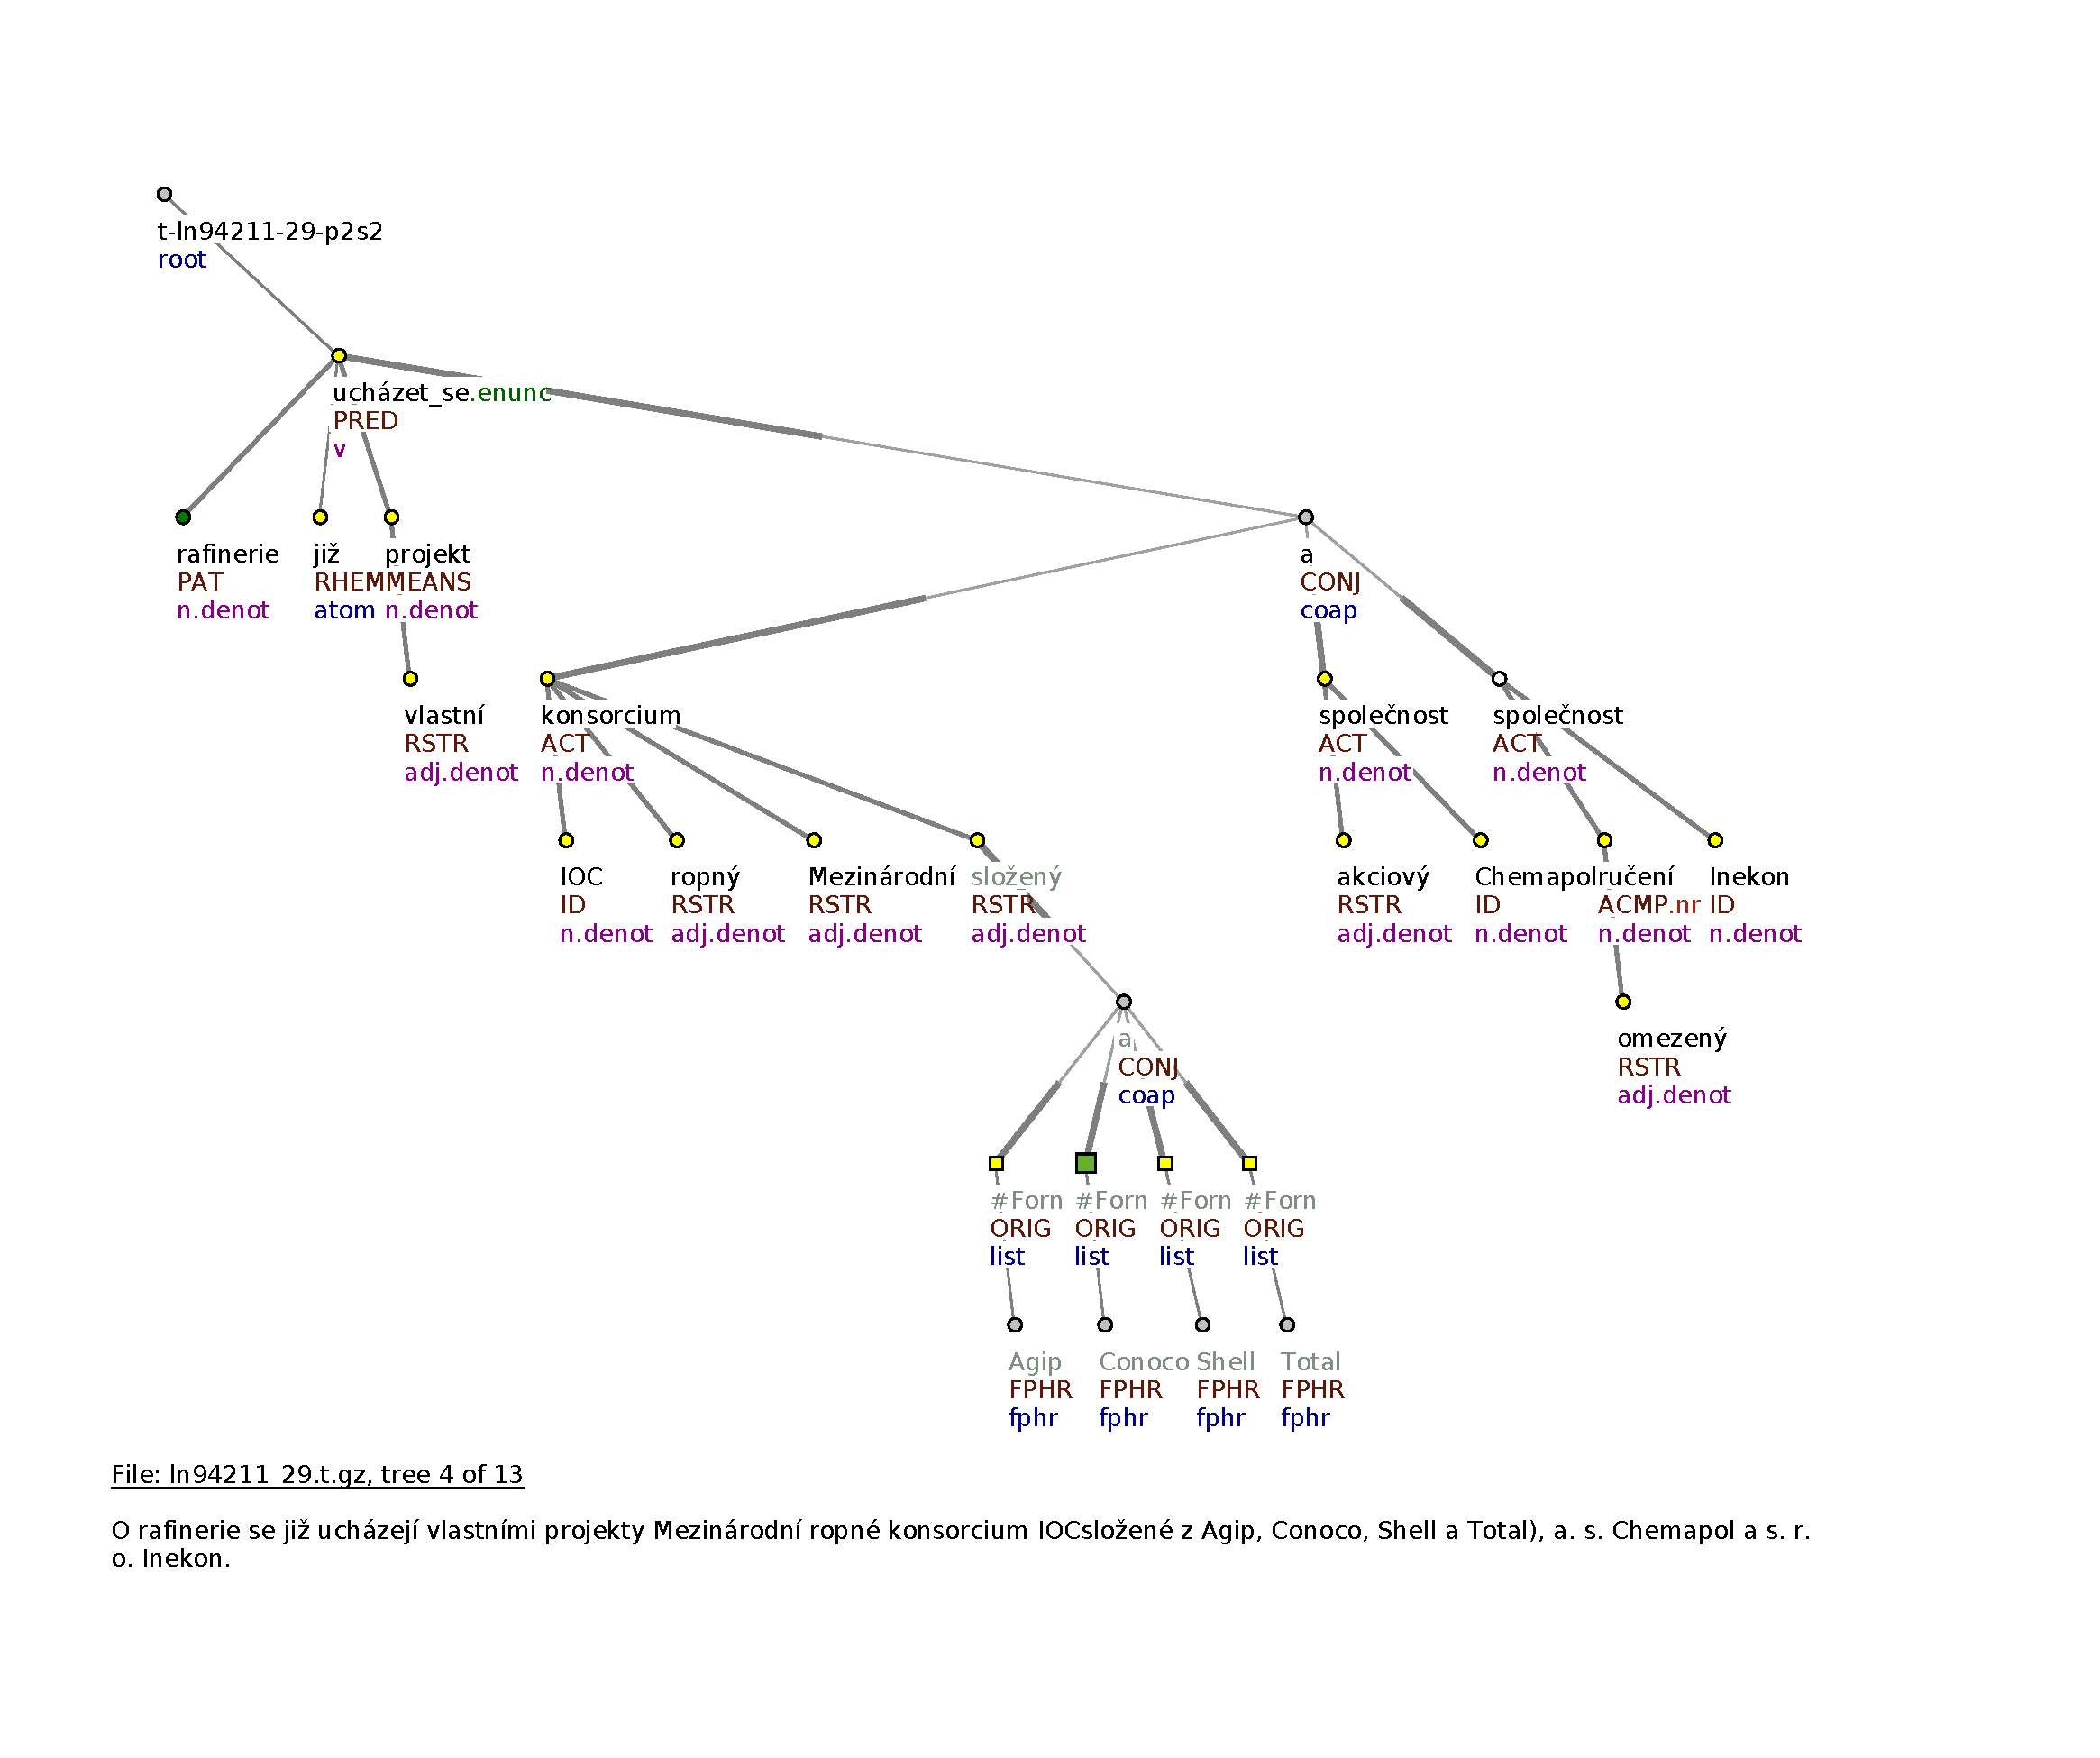
\includegraphics[width=\textwidth]{images/vyhledavky/nazvy-firem.pdf}
\caption{Annotation of Czech and foreign company names}
\label{fig:forn-firmy}
\end{figure}

%%%%%%%%%%
\section{CPHR and DPHR}

\subsection{CPHR}
There are 76 occurrences of {\tt CPHR} nodes, whose head verb is not its parent, but only effective parent, in 40 sentences. See Figure~\ref{fig:tq-echild} for the query and Figures~\ref{fig:cphr-echild} and~\ref{fig:cphr-echild2} for examples.
\begin{wrapfigure}{r}{0.32 \textwidth}
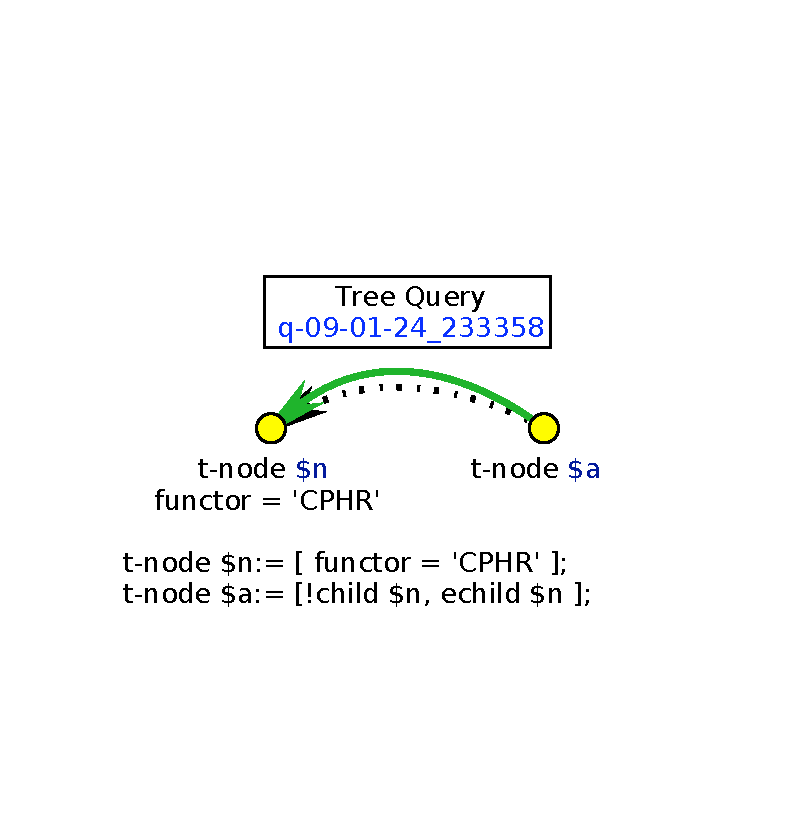
\includegraphics[width=0.3 \textwidth]{images/vyhledavky/query-echild.pdf}
\caption{PML-TQ search query for CPHR nodes, whose effective parrent is not its parent}
\label{fig:tq-echild}
\end{wrapfigure}

\begin{figure}[h]
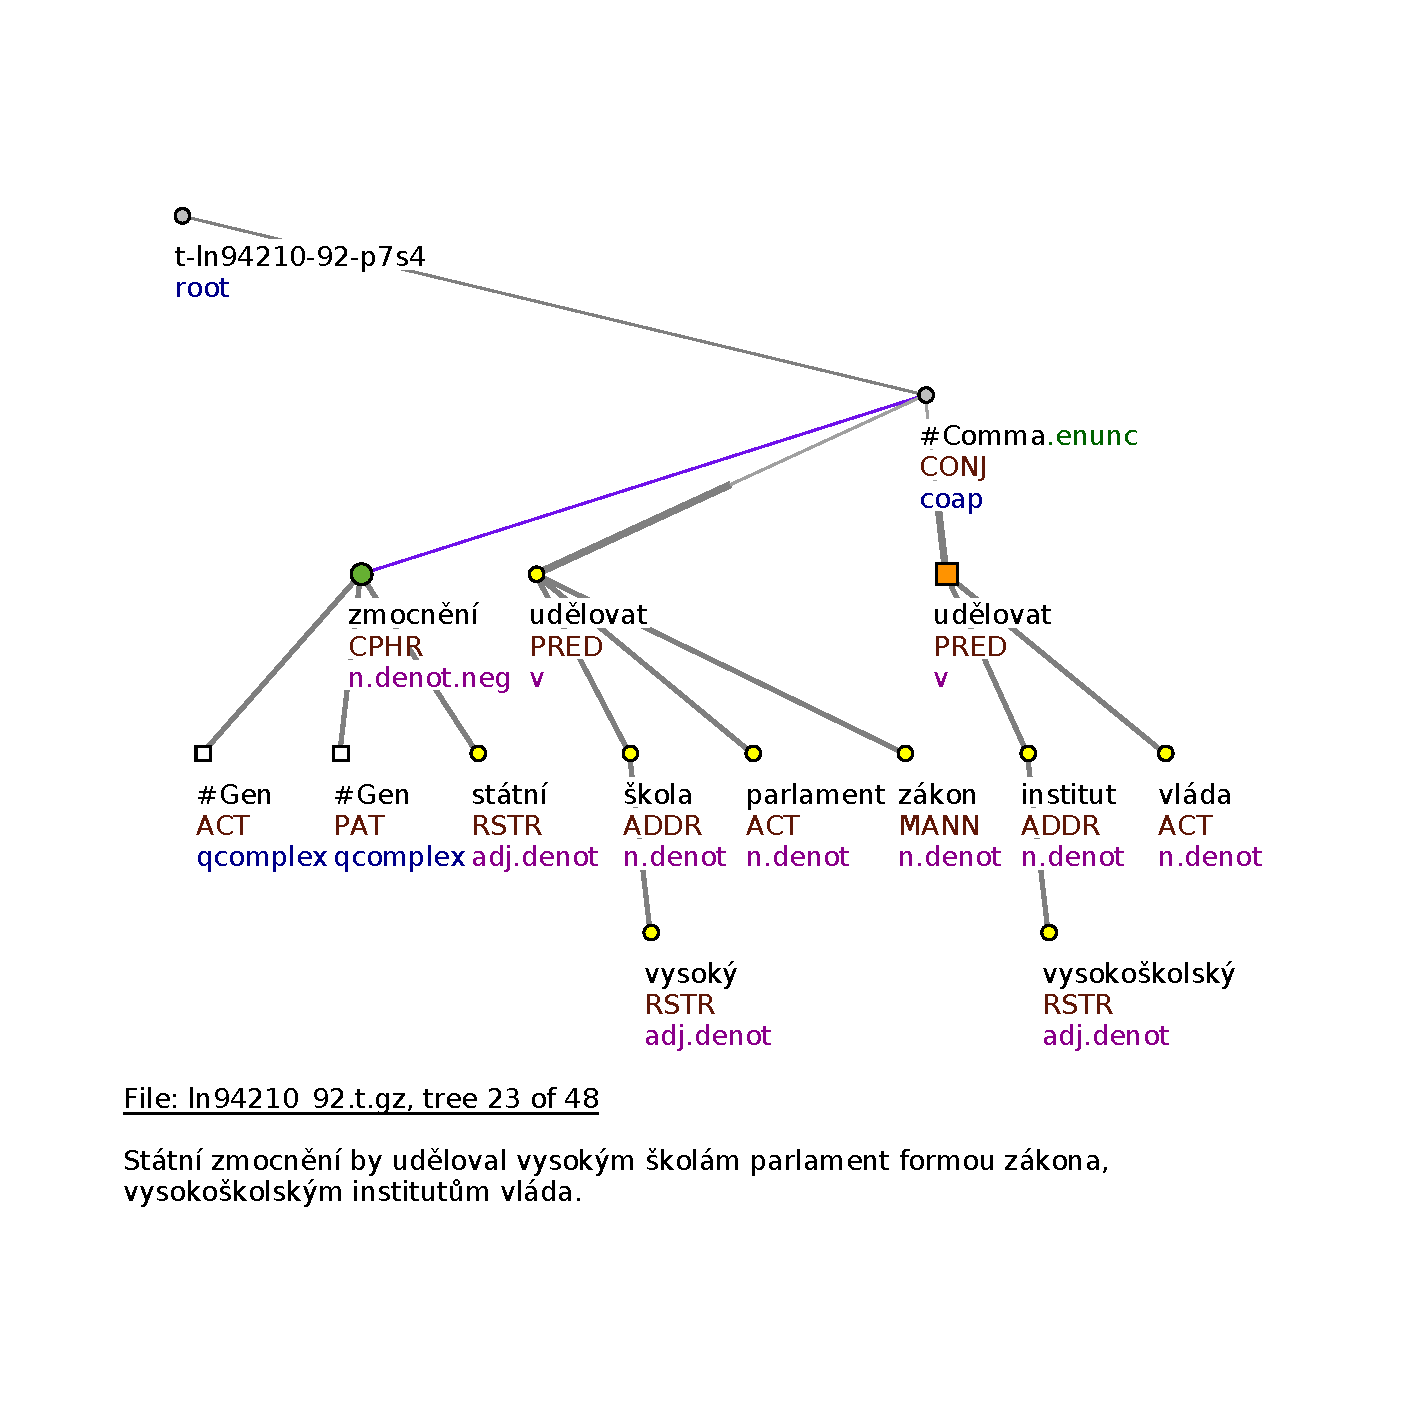
\includegraphics[width=0.8\textwidth]{images/vyhledavky/cphr-echild.pdf}
\caption{Coordination of verbonominal idioms, where the verbal parts are further ???rozvite }
\label{fig:cphr-echild}
\end{figure}

Figure~\ref{fig:cphr-echild2} shows on the other hand a coordination of two V-N idioms with the same verbal part.
\begin{figure}[h]
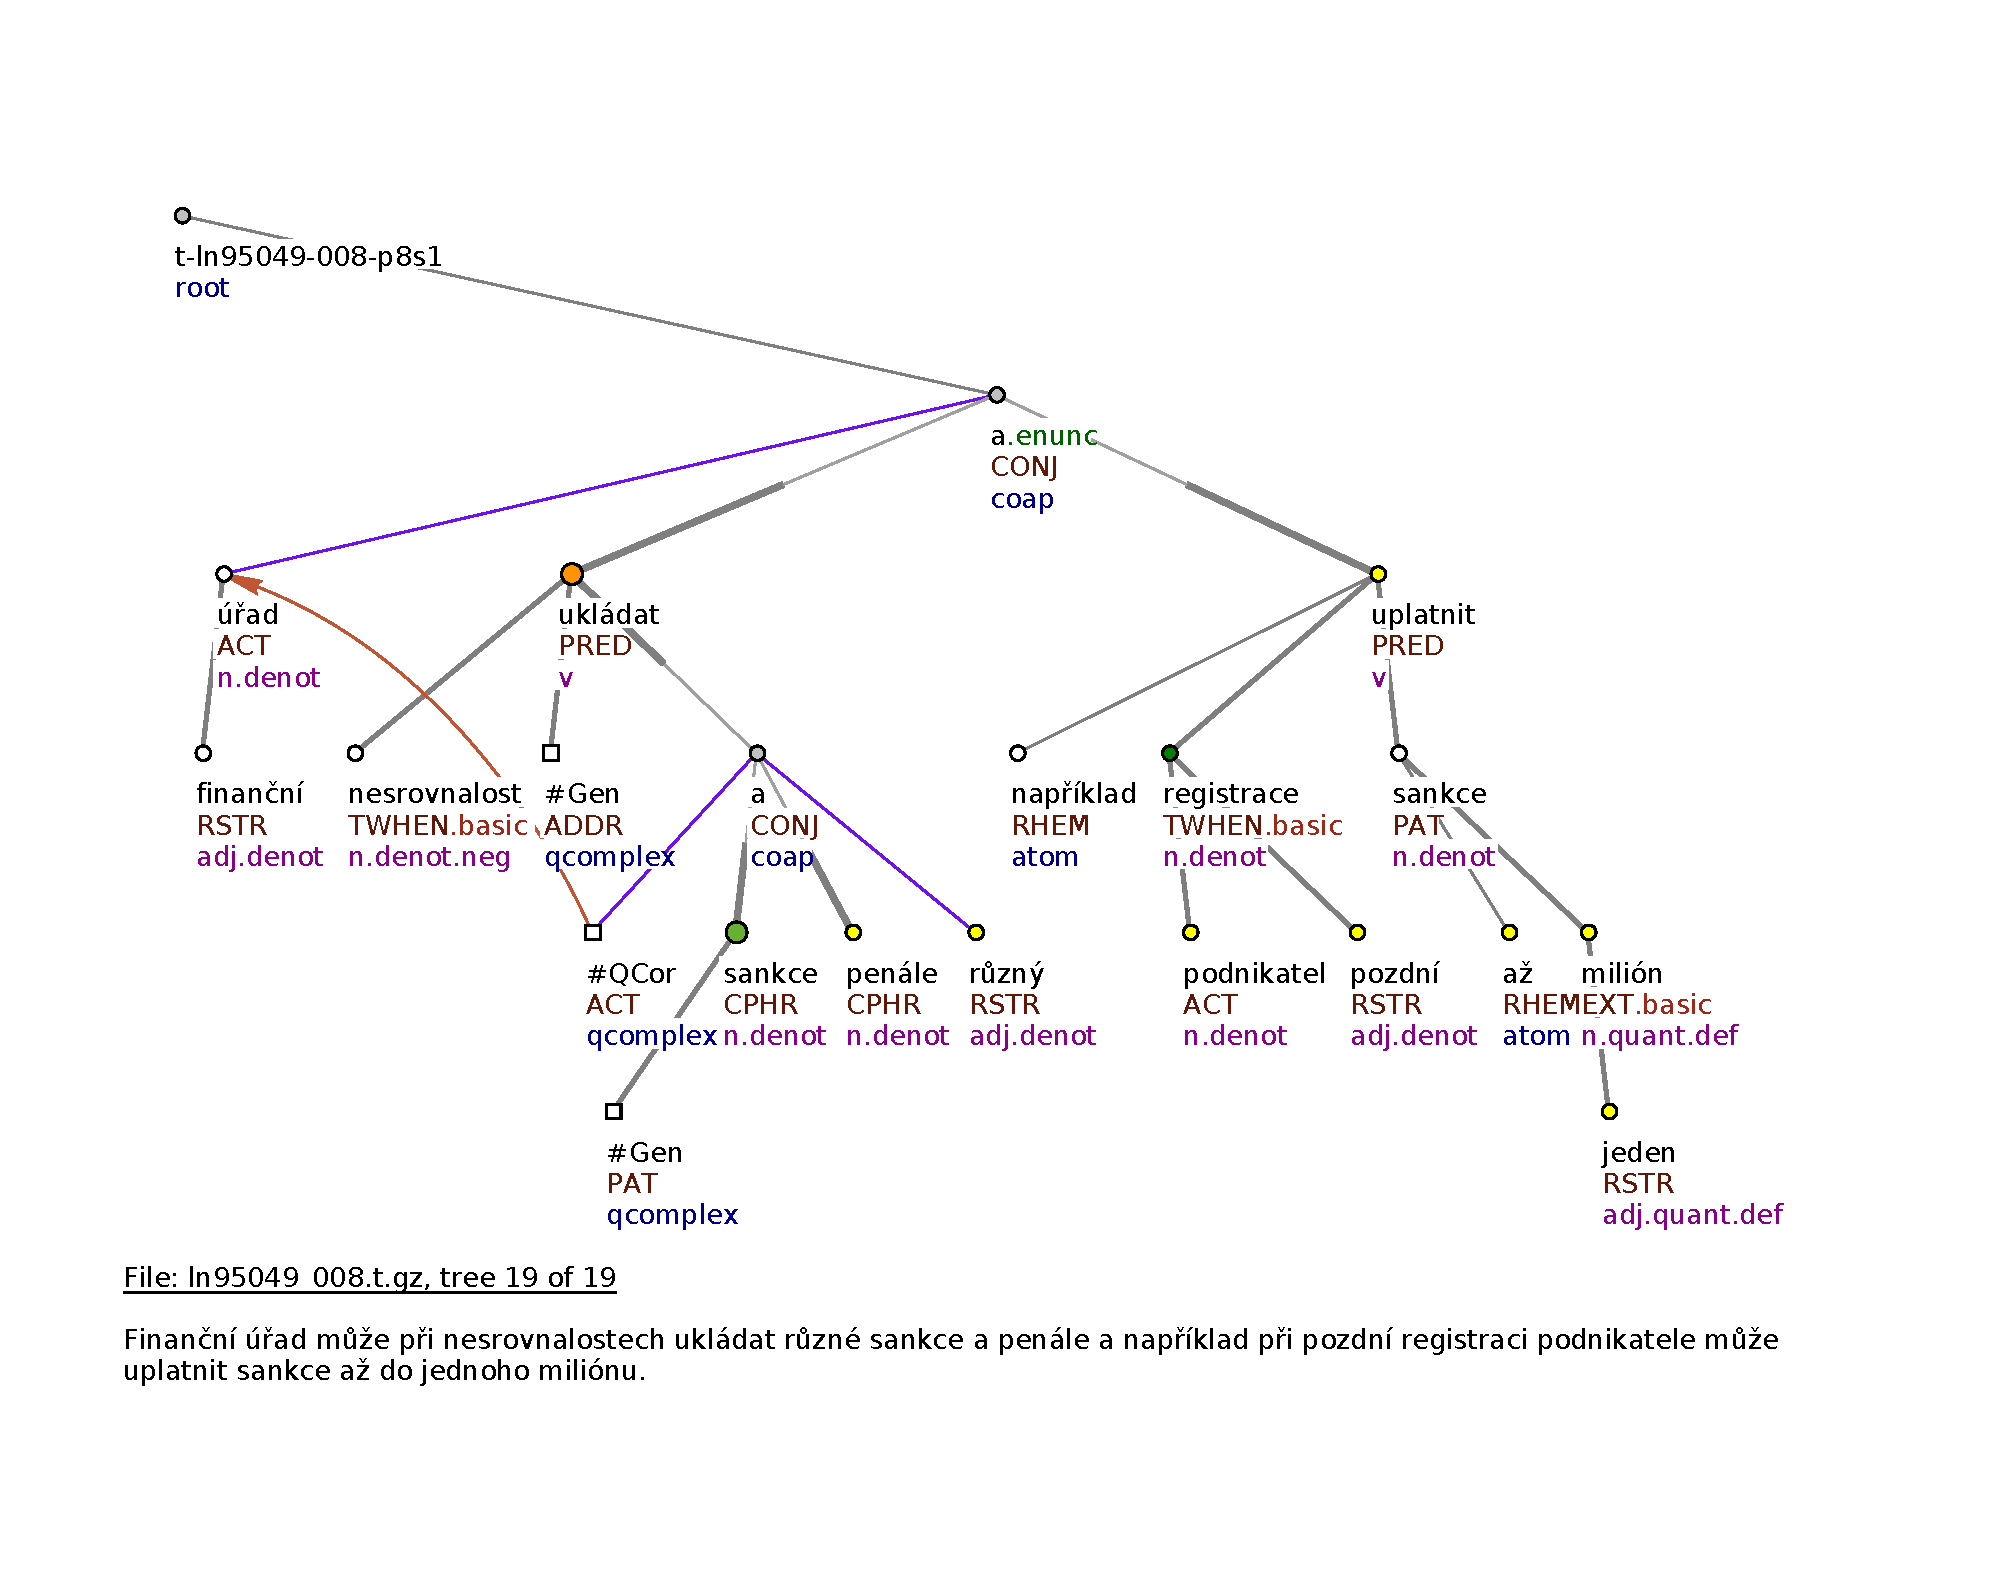
\includegraphics[width=\textwidth]{images/vyhledavky/cphr-ukladat-sankce-a-penale.pdf}
\caption{Coordination of two idioms starting with the same verb}
\label{fig:cphr-echild2}
\end{figure}


%%%%%
\section{JLRE -- Current state of MWEs in PDT 2.0}
\label{sec:pdt}
%
%\subsection{Multiword Expressions}
%\label{sec:pdt-mwe}

During the annotation of valency, which is a part of the tectogrammatical layer of PDT 2.0, the t-lemmas, have been basically identified for all the verbs and some nouns and adjectives.
The resulting valency lexicon is called PDT-VALLEX \citep{hajic:2003} and we can see it as a repository of lexemes based on verbs, adjectives and nouns in PDT that have valency.
%
\footnote{It is so because in PDT-VALLEX valency is not the only criterion for distinguishing frames (=meanings). Two words with the same morphological lemma and valency frame are assigned two different frames if their meaning differs.} 

This is a starting point for having t-nodes corresponding to lexemes. However in the current state it is not fully sufficient even for verbs, mainly because parts of MWEs are not joined into one node. Parts of frames marked as idiomatic are still represented by separate t-nodes in a tectogrammatical tree (e.g.~nodes with t-lemmas {\tt“co”} in Figure~\ref{fig:co-nevidet} or {\tt“k\_dispozici”} in Figure~\ref{fig:asistent}). Verbonominal phrasemes are also split into two nodes, where the nominal part is governed by the verb. Non-verbal idioms have not been annotated at all in the current state of PDT. 

In Figures~\ref{fig:co-nevidet}, \ref{fig:klaus}, and \ref{fig:asistent} we give several examples of t-trees in PDT 2.0, that include idioms, light verb constructions and named entities:
\begin{figure}[htbp]
   \centerline{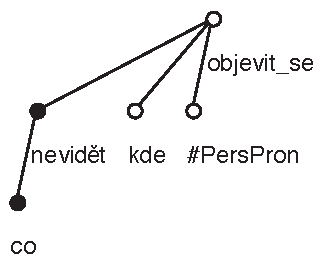
\includegraphics[scale=.7]{images/co-nevidet-clause.pdf}}
   \caption{Idiom \emph{Co nevidět} meaning ``in a blink (of an eye)'', (literally: what not-see)}
   \label{fig:co-nevidet}
\end{figure}

\begin{figure}[htbp]
   \centerline{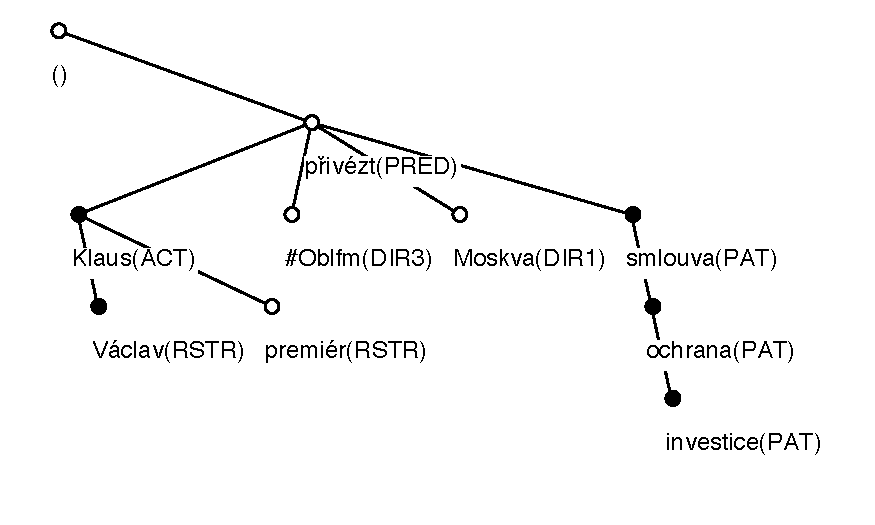
\includegraphics[width=3.7in]{images/klaus-a-smlouva.pdf}}
   \caption{A sentence featuring a personal name and a name of a bilateral treaty (which is not the exact official name, however, thus it is not capitalized)}
   \label{fig:klaus}
\end{figure}

\begin{figure}[htbp]
   \centerline{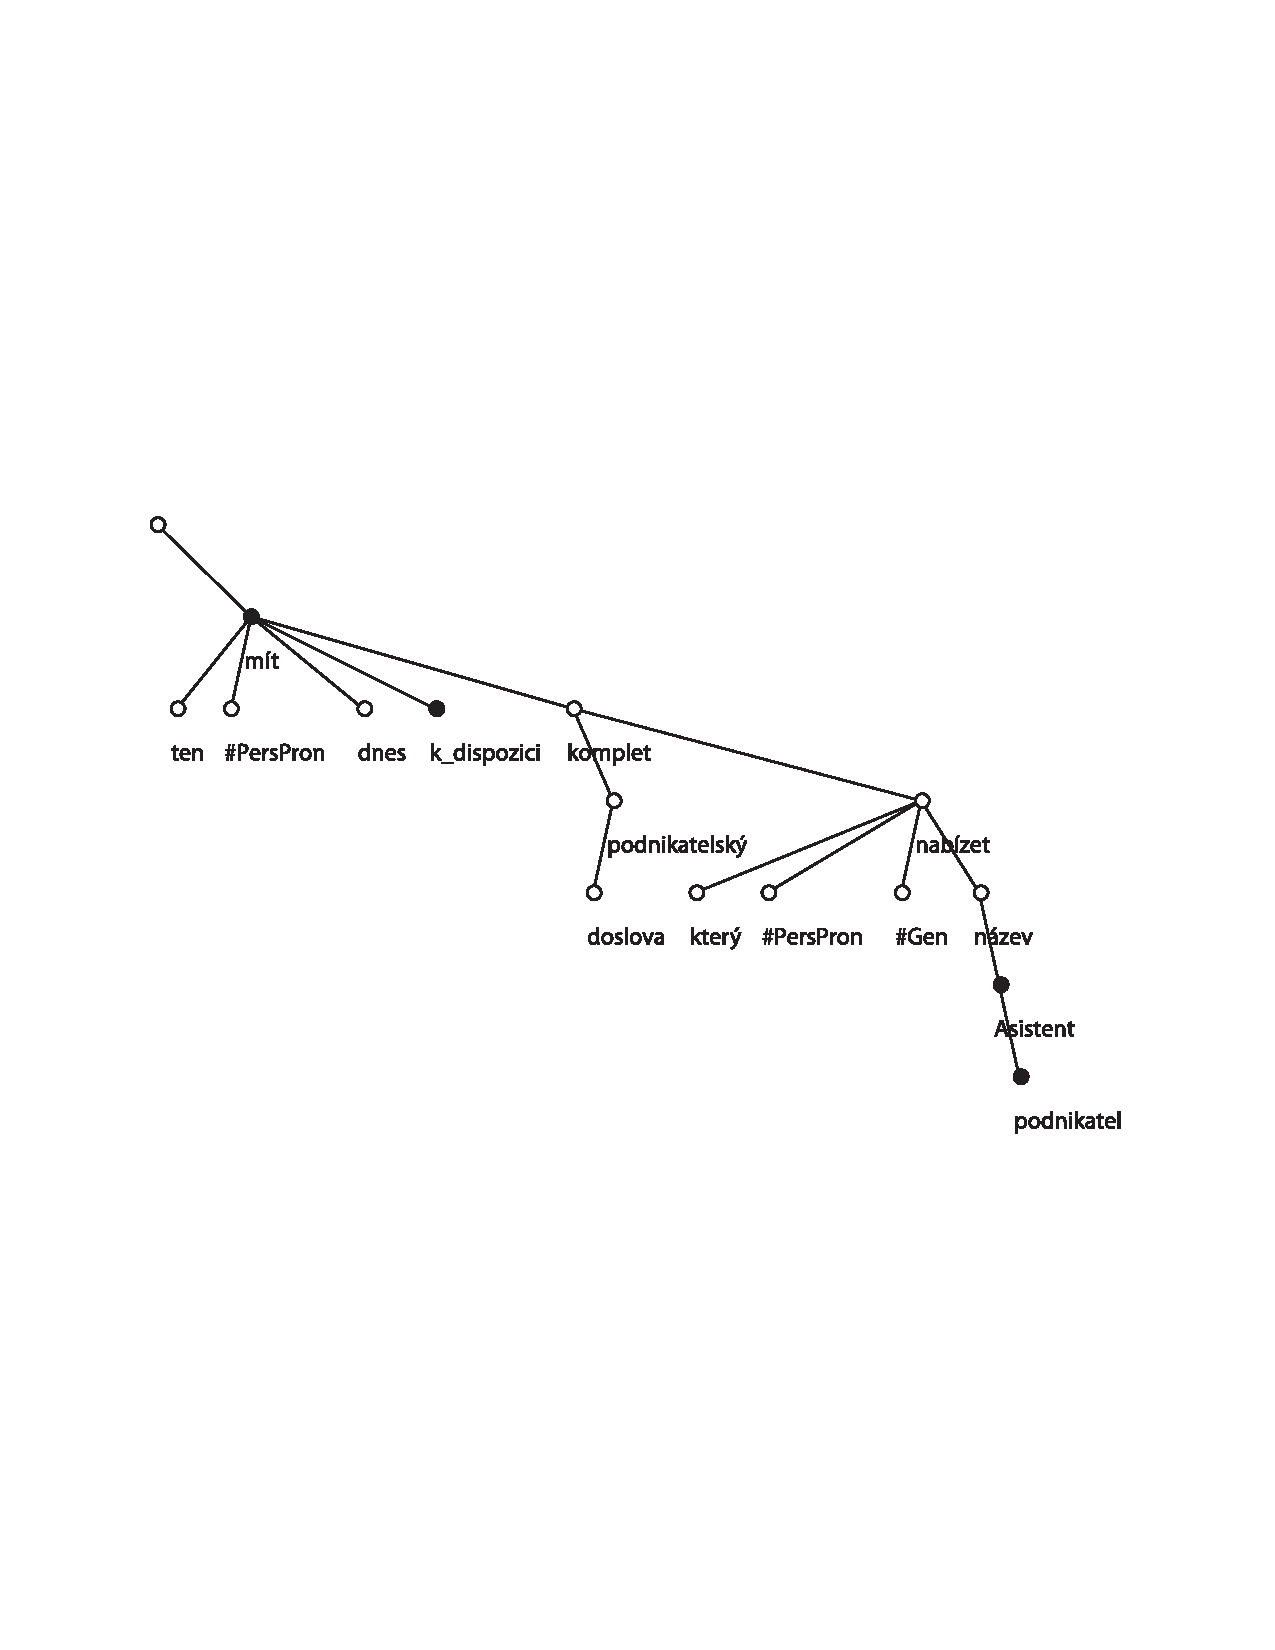
\includegraphics[height=2.6in]{images/as-pod.pdf}}
   \caption{A t-tree of a sentence featuring a light verb construction \emph{mít k dispozici} (lit.: to have at [one's] disposal) and a named entity (a product name\emph{Asistent podnikatele} (lit.: assistant of-businessman) that looks like a common phrase, except for the capital `A'.}
   \label{fig:asistent}
\end{figure}

%[[!!! doplnit informaci o seznamových strukturách s kořenem \#Idph či \#Forn.]]
